\documentclass[tikz, border=12pt]{standalone}
\usepackage[utf8]{inputenc}
\usepackage[T1]{fontenc}
\usepackage{amsmath}
\usepackage{tikz}
\usetikzlibrary{shapes.geometric, shapes.misc, arrows.meta, positioning, calc, fit, backgrounds}

\begin{document}

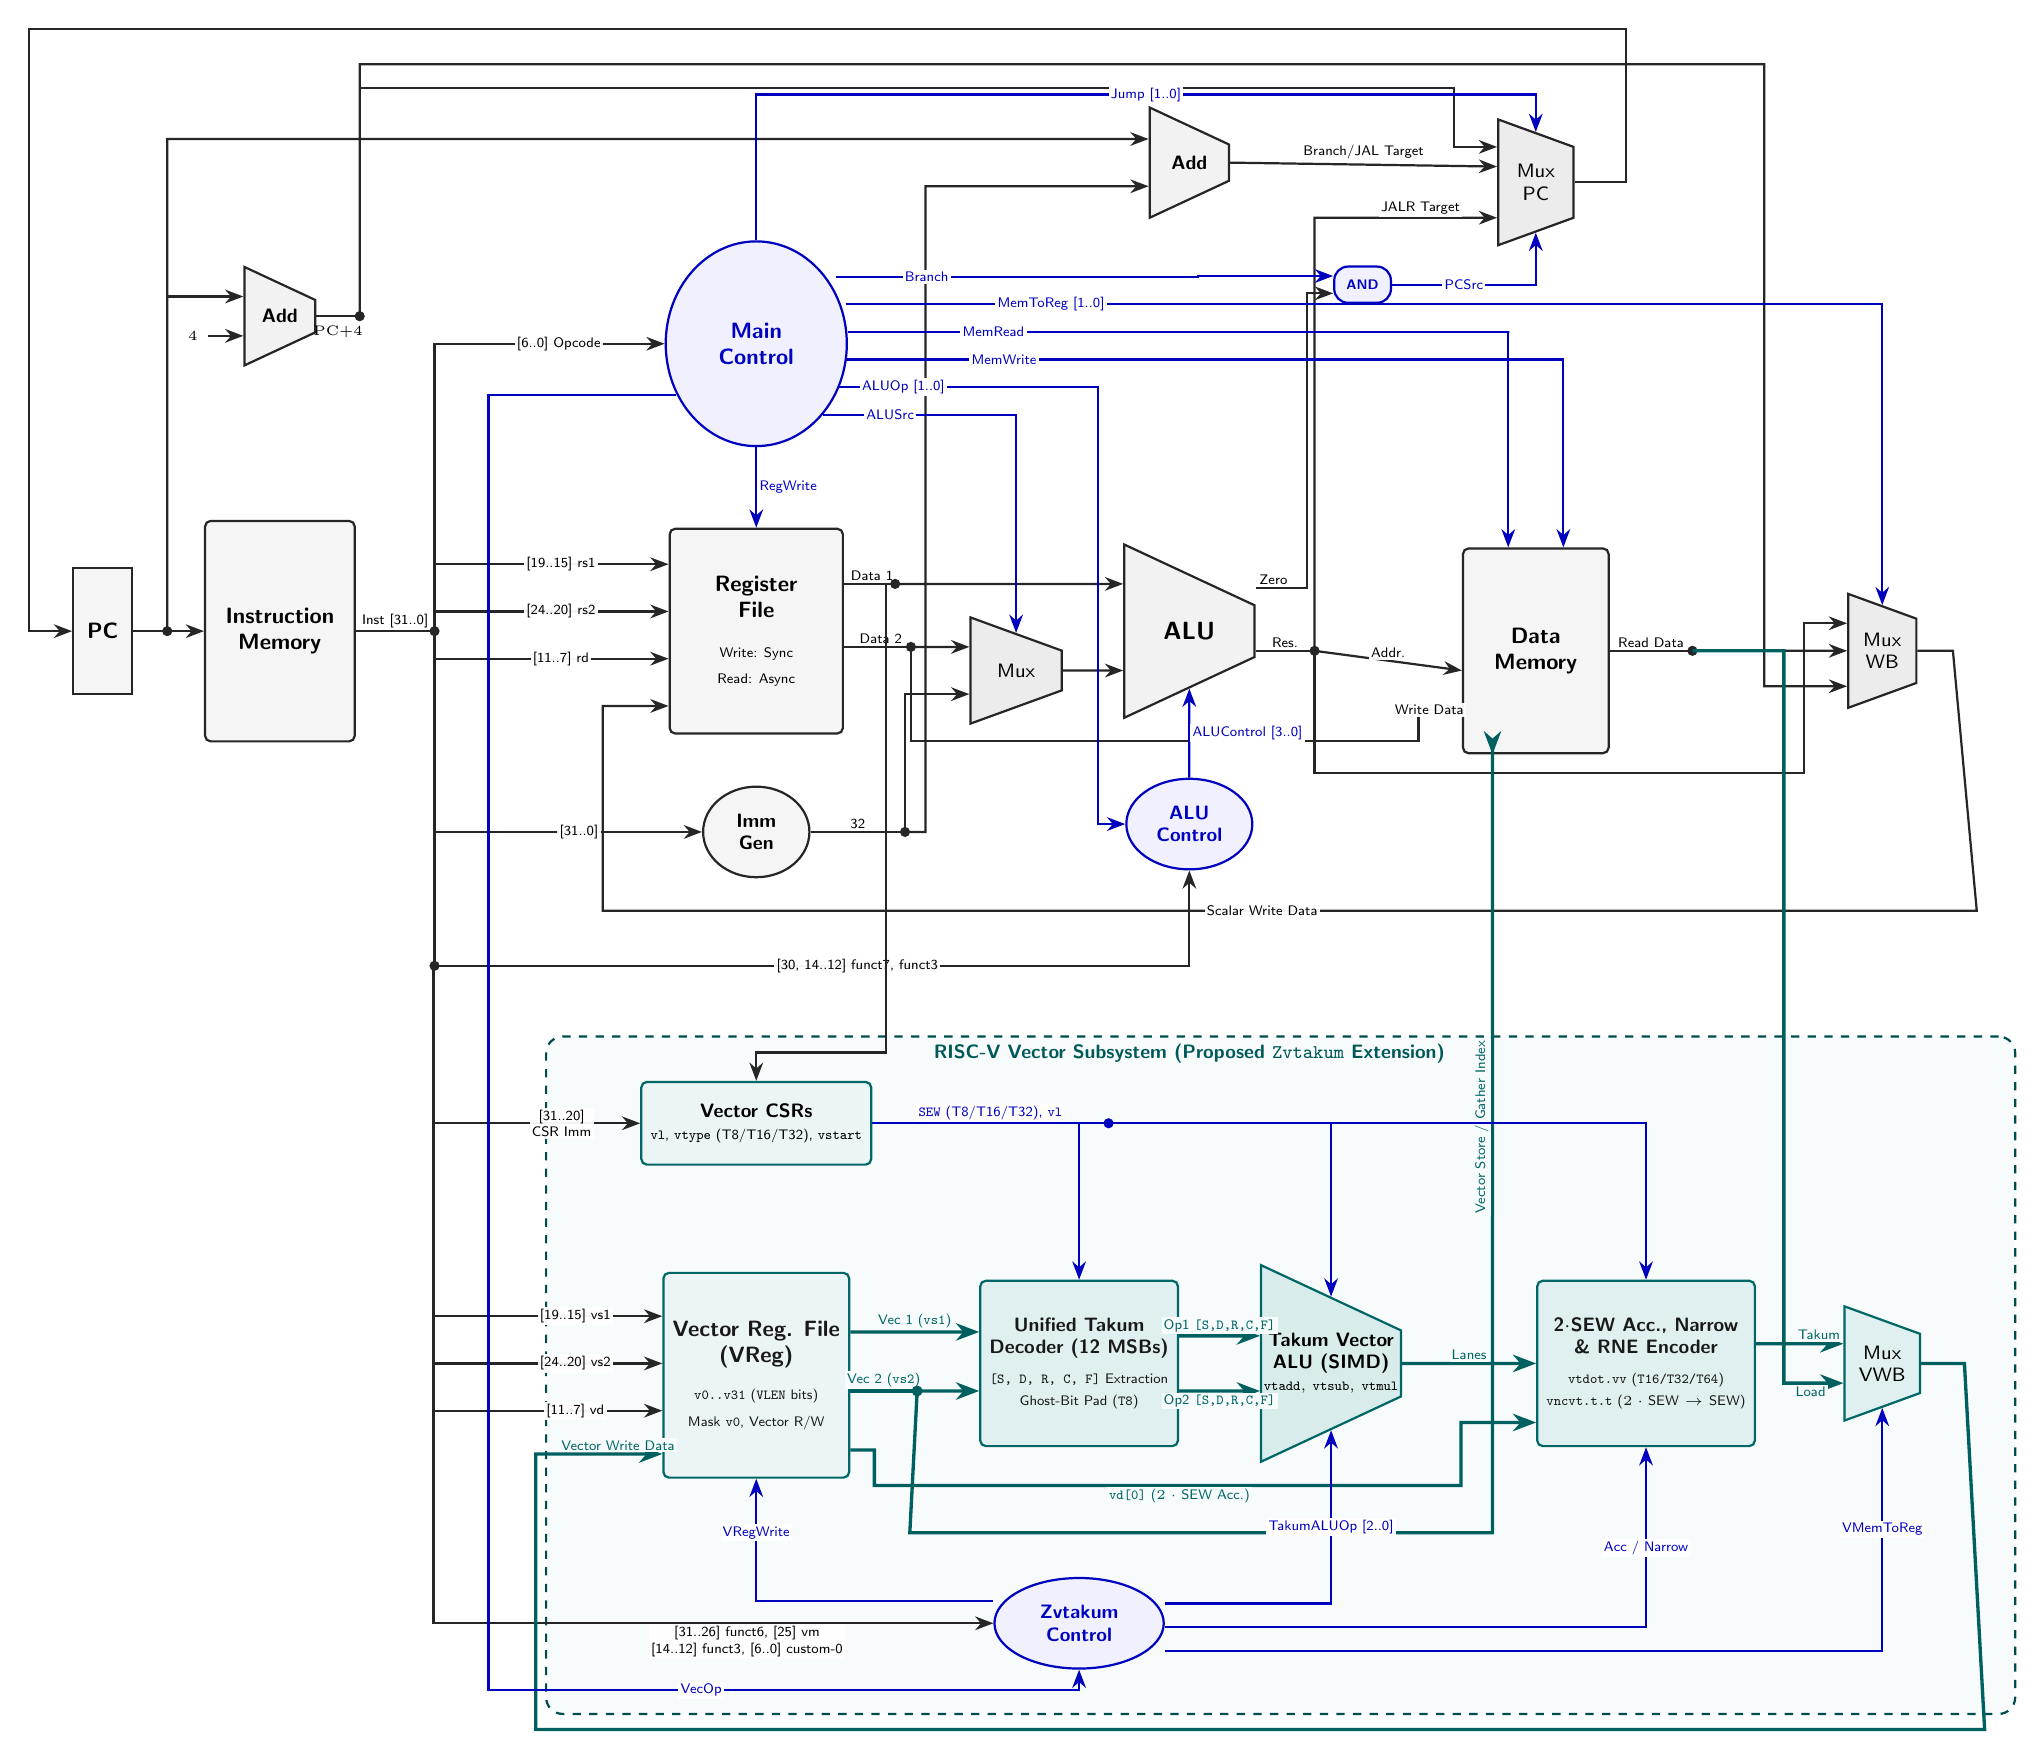
\begin{tikzpicture}[
    font=\sffamily\footnotesize,
    >=Stealth,
    % Base scalar styles
    bloco/.style={
        draw=black!85, thick, fill=gray!8,
        rectangle, minimum width=1.8cm, minimum height=2.6cm,
        align=center, rounded corners=2pt
    },
    pc_reg/.style={
        draw=black!85, thick, fill=gray!8,
        rectangle, minimum width=0.75cm, minimum height=1.6cm,
        align=center
    },
    controle/.style={
        draw=blue!75!black, thick, fill=blue!6,
        ellipse, minimum width=2.3cm, minimum height=2.6cm,
        align=center, text=blue!75!black, font=\sffamily\bfseries\footnotesize
    },
    alu_ctrl/.style={
        draw=blue!75!black, thick, fill=blue!6,
        ellipse, minimum width=1.6cm, minimum height=1.15cm,
        align=center, text=blue!75!black, font=\sffamily\bfseries\scriptsize
    },
    mux/.style={
        draw=black!85, thick, fill=gray!15,
        trapezium, trapezium angle=70, shape border rotate=270,
        minimum width=1.35cm, minimum height=0.55cm,
        inner sep=1pt, align=center, font=\sffamily\scriptsize
    },
    alu_shape/.style={
        draw=black!85, thick, fill=gray!10,
        trapezium, trapezium angle=65, shape border rotate=270,
        minimum width=2.2cm, minimum height=1.1cm,
        inner sep=1pt, align=center, font=\sffamily\bfseries\small
    },
    add_shape/.style={
        draw=black!85, thick, fill=gray!10,
        trapezium, trapezium angle=65, shape border rotate=270,
        minimum width=1.25cm, minimum height=0.75cm,
        inner sep=1pt, align=center, font=\sffamily\bfseries\scriptsize
    },
    immgen/.style={
        draw=black!85, thick, fill=gray!8,
        ellipse, minimum width=1.35cm, minimum height=1.15cm,
        align=center, font=\sffamily\scriptsize
    },
    porta_logica/.style={
        draw=blue!75!black, thick, fill=blue!6,
        rectangle, minimum width=0.72cm, minimum height=0.46cm,
        rounded corners=5pt, inner sep=1pt,
        text=blue!75!black, font=\sffamily\bfseries\tiny, align=center
    },
    % Zvtakum vector subsystem styles (teal)
    bloco_vet/.style={
        draw=teal!80!black, thick, fill=teal!8,
        rectangle, minimum width=2.2cm, minimum height=2.6cm,
        align=center, rounded corners=2pt, text=black!90
    },
    bloco_takum/.style={
        draw=teal!80!black, thick, fill=teal!12,
        rectangle, minimum width=2.25cm, minimum height=2.1cm,
        align=center, rounded corners=2pt, text=black!90, font=\sffamily\scriptsize
    },
    csr_vet/.style={
        draw=teal!80!black, thick, fill=teal!8,
        rectangle, minimum width=2.2cm, minimum height=1.05cm,
        align=center, rounded corners=2pt, font=\sffamily\scriptsize
    },
    valu_shape/.style={
        draw=teal!80!black, thick, fill=teal!15,
        trapezium, trapezium angle=65, shape border rotate=270,
        minimum width=2.3cm, minimum height=1.2cm,
        inner sep=1pt, align=center, font=\sffamily\bfseries\scriptsize
    },
    vec_ctrl/.style={
        draw=blue!75!black, thick, fill=blue!6,
        ellipse, minimum width=2.15cm, minimum height=1.15cm,
        align=center, text=blue!75!black, font=\sffamily\bfseries\scriptsize
    },
    % Wire and label styles
    fio/.style={draw=black!85, thick, ->},
    fio_sem_seta/.style={draw=black!85, thick},
    fio_vet/.style={draw=teal!75!black, very thick, ->},
    fio_vet_sem_seta/.style={draw=teal!75!black, very thick},
    fio_ctrl/.style={draw=blue!75!black, thick, ->},
    fio_ctrl_sem_seta/.style={draw=blue!75!black, thick},
    ponto/.style={fill=black!85, circle, inner sep=1.3pt},
    ponto_vet/.style={fill=teal!75!black, circle, inner sep=1.4pt},
    ponto_ctrl/.style={fill=blue!75!black, circle, inner sep=1.3pt},
    lbl/.style={font=\sffamily\tiny, fill=white, inner sep=0.8pt, opacity=0.95, text opacity=1},
    lbl_vet/.style={font=\sffamily\tiny, text=teal!80!black, fill=teal!3, inner sep=0.8pt},
    lbl_ctrl/.style={font=\sffamily\tiny, text=blue!75!black, fill=white, inner sep=0.8pt}
]

% ==========================================
% 1. SCALAR BASE DATAPATH (UPPER BAND)
% ==========================================

% Stage 1: Fetch
\node[pc_reg] (PC) at (0, 0) {\textbf{PC}};
\node[bloco, minimum width=1.9cm, minimum height=2.8cm] (MI) at (2.25, 0) {\textbf{Instruction}\\\textbf{Memory}};
\node[add_shape] (Add4) at (2.25, 4.0) {Add};

% Stage 2: Decode & Control
\node[bloco, minimum width=2.2cm] (Breg) at (8.3, 0) {
    \textbf{Register}\\\textbf{File}\\[5pt]
    {\tiny Write: Sync}\\
    {\tiny Read: Async}
};
\node[controle] (Ctrl) at (8.3, 3.65) {Main\\Control};
\node[immgen] (ImmGen) at (8.3, -2.55) {\textbf{Imm}\\\textbf{Gen}};

% Stage 3: Execute
\node[mux] (MuxULA) at (11.6, -0.5) {Mux};
\node[alu_shape] (ULA) at (13.8, 0) {ALU};
\node[alu_ctrl] (ALUCtrl) at (13.8, -2.45) {ALU\\Control};

% Branch & MuxPC (Upper Right - placed cleanly ABOVE control tracks)
\node[add_shape, minimum width=1.4cm] (AddAlvo) at (13.8, 5.95) {Add};
\node[porta_logica] (PortaAnd) at (16.0, 4.4) {AND};
\node[mux, minimum width=1.6cm] (MuxPC) at (18.2, 5.7) {Mux\\PC};

% Stage 4: Memory & Scalar Write-Back
\node[bloco, minimum width=1.85cm] (MD) at (18.2, -0.25) {\textbf{Data}\\\textbf{Memory}};
\node[mux, minimum width=1.45cm] (MuxWB) at (22.6, -0.25) {Mux\\WB};


% ==========================================
% 1B. ZVTAKUM VECTOR SUBSYSTEM (LOWER BAND)
% ==========================================

\node[csr_vet] (VCSR) at (8.3, -6.25) {
    \textbf{Vector CSRs}\\
    {\tiny \texttt{vl}, \texttt{vtype} (T8/T16/T32), \texttt{vstart}}
};

\node[bloco_vet] (VReg) at (8.3, -9.45) {
    \textbf{Vector Reg. File}\\\textbf{(VReg)}\\[4pt]
    {\tiny \texttt{v0..v31} (\texttt{VLEN} bits)}\\
    {\tiny Mask \texttt{v0}, Vector R/W}
};

\node[bloco_takum] (TakumDec) at (12.4, -9.3) {
    \textbf{Unified Takum}\\\textbf{Decoder (12 MSBs)}\\[3pt]
    {\tiny \texttt{[S, D, R, C, F]} Extraction}\\
    {\tiny Ghost-Bit Pad (\texttt{T8})}
};

\node[valu_shape] (VALU) at (15.6, -9.3) {
    Takum Vector\\ALU (SIMD)\\
    {\normalfont\tiny \texttt{vtadd}, \texttt{vtsub}, \texttt{vtmul}}
};

\node[bloco_takum, minimum width=2.45cm] (TakumAcc) at (19.6, -9.3) {
    \textbf{2$\cdot$SEW Acc., Narrow}\\\textbf{\& RNE Encoder}\\[3pt]
    {\tiny \texttt{vtdot.vv} (\texttt{T16/T32/T64})}\\
    {\tiny \texttt{vncvt.t.t} ($2\cdot\text{SEW}\to\text{SEW}$)}
};

\node[mux, draw=teal!80!black, fill=teal!12, minimum width=1.45cm] (MuxVWB) at (22.6, -9.3) {Mux\\VWB};

\node[vec_ctrl] (VecCtrl) at (12.4, -12.6) {Zvtakum\\Control};

% Highlight Frame for Zvtakum Subsystem
\begin{scope}[on background layer]
    \node[
        draw=teal!60!black, dashed, thick, fill=teal!3, rounded corners=6pt,
        fit=(VCSR) (VReg) (VecCtrl) (MuxVWB),
        inner xsep=34pt, inner ysep=16pt
    ] (BoxZvtakum) {};
    \node[
        anchor=north, align=center,
        font=\sffamily\bfseries\scriptsize, text=teal!70!black
    ] at (13.8, -5.12)
        {RISC-V Vector Subsystem (Proposed \texttt{Zvtakum} Extension)};
\end{scope}


% ==========================================
% 2. SCALAR DATA CONNECTIONS (BLACK)
% ==========================================

% PC path
\draw[fio] (PC.east) -- (MI.west);
\coordinate (JuncaoPC) at ($(PC.east)!0.48!(MI.west)$);
\node[ponto] at (JuncaoPC) {};

% PC -> Add4
\draw[fio] (JuncaoPC) |- ($(Add4.west)+(0, 0.25)$);
\draw[fio] ($(Add4.west)+(-0.45, -0.25)$) node[left, font=\tiny] {4} -- ($(Add4.west)+(0, -0.25)$);

% PC -> AddAlvo (clean corridor above Control)
\draw[fio] (JuncaoPC) -- ++(0, 6.25) -- ($(AddAlvo.west)+(-0.8, 0.3)$) -- ($(AddAlvo.west)+(0, 0.3)$);

% PC+4 output
\coordinate (SaidaPC4) at ($(Add4.east)+(0.55, 0)$);
\draw[fio_sem_seta] (Add4.east) -- node[below, font=\tiny] {PC+4} (SaidaPC4);
\node[ponto] at (SaidaPC4) {};

% PC+4 -> MuxPC (top channel)
\draw[fio] (SaidaPC4) -- ++(0, 2.9) -| ($(MuxPC.west)+(-0.55, 0.45)$) -- ($(MuxPC.west)+(0, 0.45)$);

% PC+4 -> MuxWB (runs above MuxPC and drops in clean corridor between MD and MuxWB)
\draw[fio] (SaidaPC4) -- ++(0, 3.2) -- (21.1, 7.2) -- (21.1, -0.7) -- ($(MuxWB.west)+(0, -0.45)$);

% MuxPC -> PC feedback
\draw[fio] (MuxPC.east) -- ++(0.65, 0) -- ++(0, 1.95) -| ($(PC.west)+(-0.55, 0)$) -- (PC.west);

% Instruction Bus (32 bits)
\coordinate (BusInst) at ($(MI.east)+(1.0, 0)$);
\draw[fio_sem_seta] (MI.east) -- node[lbl, above] {Inst [31..0]} (BusInst);
\node[ponto] at (BusInst) {};

\draw[fio] (BusInst) |- node[lbl, pos=0.77] {[6..0] Opcode} (Ctrl.west);
\draw[fio] (BusInst) |- node[lbl, pos=0.77] {[19..15] rs1} ($(Breg.west)+(0, 0.85)$);
\draw[fio] (BusInst) |- node[lbl, pos=0.77] {[24..20] rs2} ($(Breg.west)+(0, 0.25)$);
\draw[fio] (BusInst) |- node[lbl, pos=0.77] {[11..7] rd} ($(Breg.west)+(0, -0.35)$);
\draw[fio] (BusInst) |- node[lbl, pos=0.77] {[31..0]} (ImmGen.west);

% Drop to ALUControl cleanly at y = -4.25 (separate from Write-Back wire at y = -3.55)
\coordinate (BusInstALU) at ($(BusInst)+(0, -4.25)$);
\draw[fio_sem_seta] (BusInst) -- (BusInstALU);
\node[ponto] at (BusInstALU) {};
\draw[fio] (BusInstALU) -| node[lbl, pos=0.28] {[30, 14..12] funct7, funct3} (ALUCtrl.south);

% Scalar Register File outputs
\coordinate (SaidaDado1) at ($(Breg.east)+(0.65, 0.6)$);
\draw[fio_sem_seta] ($(Breg.east)+(0, 0.6)$) -- node[lbl, above, pos=0.55] {Data 1} (SaidaDado1);
\node[ponto] at (SaidaDado1) {};
\draw[fio] (SaidaDado1) -- ($(ULA.west)+(0, 0.6)$);

\coordinate (Dado2) at ($(Breg.east)+(0, -0.2)$);
\coordinate (JuncaoDado2) at ($(Dado2)+(0.85, 0)$);
\draw[fio_sem_seta] (Dado2) -- node[lbl, above, pos=0.55] {Data 2} (JuncaoDado2);
\node[ponto] at (JuncaoDado2) {};
\draw[fio] (JuncaoDado2) -- ($(MuxULA.west)+(0, 0.3)$);

% Data 2 -> Data Memory (Write Data)
\draw[fio] (JuncaoDado2) -- ++(0, -1.2) -| ($(MD.west)+(-0.55, -0.75)$) -- node[lbl, pos=0.25] {Write Data} ($(MD.west)+(0, -0.75)$);

% ImmGen output
\coordinate (SaidaImm) at ($(ImmGen.east)+(1.2, 0)$);
\draw[fio_sem_seta] (ImmGen.east) -- node[lbl, above] {32} (SaidaImm);
\node[ponto] at (SaidaImm) {};

\draw[fio] (SaidaImm) |- ($(MuxULA.west)+(0, -0.3)$);
% Imm -> AddAlvo via clean corridor at x = 10.45
\draw[fio] (SaidaImm) -- (10.45, -2.55) -- (10.45, 5.65) -- ($(AddAlvo.west)+(0, -0.3)$);

% AddAlvo -> MuxPC
\draw[fio] (AddAlvo.east) -- node[lbl, above, yshift=1pt] {Branch/JAL Target} ($(MuxPC.west)+(0, 0.2)$);

% Scalar ALU execution
\draw[fio] (MuxULA.east) -- ($(ULA.west)+(0, -0.5)$);
\draw[fio] ($(ULA.east)+(0, 0.55)$) -- node[lbl, pos=0.35, above] {Zero} ++(0.65, 0) |- ($(PortaAnd.west)+(0, -0.11)$);

\coordinate (SaidaULA) at ($(ULA.east)+(0.75, -0.25)$);
\draw[fio_sem_seta] ($(ULA.east)+(0, -0.25)$) -- node[lbl, above] {Res.} (SaidaULA);
\node[ponto] at (SaidaULA) {};

\draw[fio] (SaidaULA) -- node[lbl, above] {Addr.} ($(MD.west)+(0, -0.25)$);
\draw[fio] (SaidaULA) -- ++(0, -1.55) -| ($(MuxWB.west)+(-0.55, 0.35)$) -- ($(MuxWB.west)+(0, 0.35)$);
\draw[fio] (SaidaULA) -- ++(0, 5.5) -- node[lbl, pos=0.72, above] {JALR Target} ($(MuxPC.west)+(-0.45, -0.45)$) -- ($(MuxPC.west)+(0, -0.45)$);

% Data Memory -> MuxWB
\coordinate (SaidaMD) at ($(MD.east)+(1.05, 0.0)$);
\draw[fio_sem_seta] ($(MD.east)+(0, 0.0)$) -- node[lbl, above] {Read Data} (SaidaMD);
\node[ponto] at (SaidaMD) {};
\draw[fio] (SaidaMD) -- ($(MuxWB.west)+(0, 0.0)$);

% Scalar Write-Back (at y = -3.55, cleanly ABOVE BusInstALU at y = -4.25)
\draw[fio] (MuxWB.east) -- ++(0.45, 0) -- (23.8, -3.55) -- node[lbl, pos=0.52] {Scalar Write Data} (6.35, -3.55) -- (6.35, -0.95) -- ($(Breg.west)+(0, -0.95)$);


% ==========================================
% 2B. VECTOR DATA CONNECTIONS (TEAL/BLACK)
% ==========================================

% Instruction Bus -> Zvtakum Subsystem (left channel x = 4.2)
\coordinate (BusInstVec) at (4.2, -4.25);
\draw[fio_sem_seta] (BusInstALU) -- (BusInstVec);
\draw[fio] (BusInstVec) |- node[lbl, pos=0.81, align=center] {[31..20]\\CSR Imm} (VCSR.west);
\draw[fio] (BusInstVec) |- node[lbl, pos=0.81] {[19..15] vs1} ($(VReg.west)+(0, 0.75)$);
\draw[fio] (BusInstVec) |- node[lbl, pos=0.81] {[24..20] vs2} ($(VReg.west)+(0, 0.15)$);
\draw[fio] (BusInstVec) |- node[lbl, pos=0.81] {[11..7] vd} ($(VReg.west)+(0, -0.45)$);
\draw[fio] (BusInstVec) |- node[lbl, pos=0.78, below, align=center] {[31..26] funct6, [25] vm\\{[14..12] funct3, [6..0] custom-0}} (VecCtrl.west);

% Scalar Data 1 (rs1) -> Vector CSRs (corridor x = 9.95, cleanly to the left of title at x=13.8)
\draw[fio] (SaidaDado1) -- (9.95, 0.6) -- (9.95, -5.35) -| (VCSR.north);

% VReg -> Takum Decoder (vs1, vs2)
\draw[fio_vet] ($(VReg.east)+(0, 0.55)$) -- node[lbl_vet, above] {Vec 1 (\texttt{vs1})} ($(TakumDec.west)+(0, 0.4)$);

\coordinate (SaidaVet2) at ($(VReg.east)+(0.85, -0.2)$);
\draw[fio_vet_sem_seta] ($(VReg.east)+(0, -0.2)$) -- node[lbl_vet, above] {Vec 2 (\texttt{vs2})} (SaidaVet2);
\node[ponto_vet] at (SaidaVet2) {};
\draw[fio_vet] (SaidaVet2) -- ($(TakumDec.west)+(0, -0.35)$);

% VReg -> Extended Accumulator vd[0] (2*SEW for vtdot.vv) at y = -10.85
\draw[fio_vet] ($(VReg.east)+(0, -0.95)$) -- (9.8, -10.4) -- (9.8, -10.85) -- (17.25, -10.85)
    node[lbl_vet, pos=0.52, below] {\texttt{vd[0]} ($2\cdot\text{SEW}$ Acc.)}
    |- ($(TakumAcc.west)+(0, -0.75)$);

% Vec 2 (vs2) / Gather indices -> Data Memory via corridor x = 17.65 (between VALU and TakumAcc)
\draw[fio_vet] (SaidaVet2) -- (10.25, -11.45) -- (17.65, -11.45) -- (17.65, -1.55)
    node[lbl_vet, pos=0.52, rotate=90, above] {Vector Store / Gather Index}
    -- ($(MD.south)+(-0.55, 0)$);

% Takum Decoder -> Vector Takum ALU
\draw[fio_vet] ($(TakumDec.east)+(0, 0.35)$) -- node[lbl_vet, above] {Op1 \texttt{[S,D,R,C,F]}} ($(VALU.west)+(0, 0.35)$);
\draw[fio_vet] ($(TakumDec.east)+(0, -0.35)$) -- node[lbl_vet, below] {Op2 \texttt{[S,D,R,C,F]}} ($(VALU.west)+(0, -0.35)$);

% VALU -> Accumulator/Encoder
\draw[fio_vet] (VALU.east) -- node[lbl_vet, above] {Lanes} (TakumAcc.west);

% Accumulator/Encoder -> MuxVWB (0)
\draw[fio_vet] ($(TakumAcc.east)+(0, 0.25)$) -- node[lbl_vet, above, pos=0.72] {Takum} ($(MuxVWB.west)+(0, 0.25)$);

% Data Memory Read Data -> MuxVWB (1 - Vector Load, corridor x = 21.35)
\draw[fio_vet] (SaidaMD) -- (21.35, -0.25) -- (21.35, -9.55) -- node[lbl_vet, below, pos=0.45] {Load} ($(MuxVWB.west)+(0, -0.25)$);

% Vector Write-Back: MuxVWB -> VReg (bottom return track at y = -13.95)
\draw[fio_vet] (MuxVWB.east) -- ++(0.55, 0) -- (23.9, -13.95) -- (5.5, -13.95) -- (5.5, -10.45) -- node[lbl_vet, pos=0.65, above] {Vector Write Data} ($(VReg.west)+(0, -1.0)$);


% ==========================================
% 3. CONTROL SIGNALS (BLUE - CLEAN TRACKS)
% ==========================================

% Track 0 (Top): Jump [1..0] -> MuxPC (above AddAlvo)
\draw[fio_ctrl] (Ctrl.north) -- ++(0, 1.85) -| node[lbl_ctrl, pos=0.25] {Jump [1..0]} (MuxPC.north);

% Branch -> AND gate
\draw[fio_ctrl] ($(Ctrl.east)+(-0.15, 0.85)$) -- node[lbl_ctrl, pos=0.25] {Branch} ++(4.6, 0) |- ($(PortaAnd.west)+(0, 0.11)$);

% AND -> MuxPC (PCSrc)
\draw[fio_ctrl] (PortaAnd.east) -| node[lbl_ctrl, pos=0.25] {PCSrc} (MuxPC.south);

% Stacked horizontal tracks cleanly BELOW AddAlvo and ABOVE ULA/MD
\draw[fio_ctrl] ($(Ctrl.east)+(-0.02, 0.50)$) -- node[lbl_ctrl, pos=0.20] {MemToReg [1..0]} ++(13.0, 0) -| (MuxWB.north);
\draw[fio_ctrl] ($(Ctrl.east)+(0.0, 0.15)$) -- node[lbl_ctrl, pos=0.22] {MemRead} ++(8.4, 0) -| ($(MD.north)+(-0.35, 0)$);
\draw[fio_ctrl] ($(Ctrl.east)+(-0.02, -0.20)$) -- node[lbl_ctrl, pos=0.22] {MemWrite} ++(9.1, 0) -| ($(MD.north)+(0.35, 0)$);
\draw[fio_ctrl] ($(Ctrl.east)+(-0.12, -0.55)$) -- node[lbl_ctrl, pos=0.25] {ALUOp [1..0]} ++(3.3, 0) |- (ALUCtrl.west);
\draw[fio_ctrl] ($(Ctrl.east)+(-0.32, -0.90)$) -- node[lbl_ctrl, pos=0.35] {ALUSrc} ++(2.45, 0) -| (MuxULA.north);

% RegWrite -> Register File
\draw[fio_ctrl] (Ctrl.south) -- node[lbl_ctrl, right] {RegWrite} (Breg.north);

% ALU Control -> ALU
\draw[fio_ctrl] (ALUCtrl.north) -- node[lbl_ctrl, right] {ALUControl [3..0]} (ULA.south);

% --- Zvtakum Control Signals ---
% Main Control -> VecCtrl (outer left route at x = 4.9)
\draw[fio_ctrl] ($(Ctrl.west)+(0.15, -0.65)$) -- (4.9, 3.0) -- (4.9, -13.45) -| node[lbl_ctrl, pos=0.18] {VecOp} (VecCtrl.south);

% Vector CSRs (SEW, vl) -> TakumDec, VALU, TakumAcc along horizontal bus y = -6.25
\coordinate (SaidaSEW) at ($(VCSR.east)+(3.0, 0)$);
\draw[fio_ctrl_sem_seta] (VCSR.east) -- node[lbl_ctrl, above] {\texttt{SEW} (T8/T16/T32), \texttt{vl}} (SaidaSEW);
\node[ponto_ctrl] at (SaidaSEW) {};
\draw[fio_ctrl] (SaidaSEW) -| (TakumDec.north);
\draw[fio_ctrl] (SaidaSEW) -| (VALU.north);
\draw[fio_ctrl] (SaidaSEW) -| (TakumAcc.north);

% VecCtrl -> VReg, VALU, TakumAcc, MuxVWB
\draw[fio_ctrl] ($(VecCtrl.west)+(0, 0.28)$) -| node[lbl_ctrl, pos=0.78] {VRegWrite} (VReg.south);
\draw[fio_ctrl] ($(VecCtrl.east)+(0, 0.25)$) -| node[lbl_ctrl, pos=0.72] {TakumALUOp [2..0]} (VALU.south);
\draw[fio_ctrl] ($(VecCtrl.east)+(0, -0.05)$) -| node[lbl_ctrl, pos=0.72] {Acc / Narrow} (TakumAcc.south);
\draw[fio_ctrl] ($(VecCtrl.east)+(0, -0.35)$) -| node[lbl_ctrl, pos=0.75] {VMemToReg} (MuxVWB.south);

\end{tikzpicture}
\end{document}
